%%%%%%%%%%%%%%%%%%%%%%%%%%%%%%%%%%%%%%%%%%%%%%%%%%%%%%%%%%%%%%%%%%%%%%%%%%%%%%%%
%%%
%%% Введение
%%%

\subsection{Построение сетевой модели}

Сложность и~комплексность разработки и~реализации описанного проекта, 
необходимость параллельного выполнения работ, 
зависимость начала многих работ от результатов других, 
значительно осложняют планирование разработки.

При наличии множества взаимосвязанных работ,
наиболее удобными являются системы сетевого планирования и~управления (СПУ).
Они основаны на~применении сетевых моделей планируемых процессов, 
которые допускают использование современной вычислительной техники. 

Сетевые модели планируемых процессов позволяют быстро определить 
последствия различных вариантов управляющих 
воздействий и~находить наилучшие из них. 

СПУ дают возможность своевременно получать достоверную информацию о~состоянии дел, 
о возникших задержках и~возможностях ускорения хода работ, 
концентрируют внимание на~<<критических>> работах, 
определяющих продолжительность проведения разработки в целом, 
заставляют совершенствовать технологию и~организацию работ, 
непосредственно влияющих на~сроки проведения разработки, 
помогают составлять рациональные планы работ.

\subsubsection{Перечень работ и~событий}

Составим полный перечень событий и~работ сетевой модели. 
Каждая работа имеет определенную продолжительность. 
Однако не всегда заранее известно точное время выполнения работ, 
поэтому дадим продолжительности каждой работы две вероятностные оценки:   

\begin{itemize}
	\item минимальную (оптимистическую) --- $t_{min}$;
	\item максимальную (пессимистическую) --- $t_{max}$.
\end{itemize}

Эти величины являются исходными для расчета ожидаемого времени выполнения работ:  .
\[
	t_{\text{ожидаемое}} = \dfrac{3 \cdot t_{min} + 2 \cdot t_{max} }{5}
\]

Рассчитаем дисперсии работ по формуле:   
\[
	\delta^2 = \left(  \dfrac{ t_{max} - t_{min} }{5} \right)^2
\]




\pagebreak


{ \footnotesize \sffamily 
\begin{spacing}{1.2}
\begin{center}
	\captionsetup{font=rm,justification=raggedleft, singlelinecheck=false,font=small}
	\newcommand{\headlinetext}{
		\textbf{№} &	\textbf{Наименование события}  &	\textbf{Код работы}  &	\textbf{Наименование  работы} 
		& $\mathbf{t_{min}}$ &	$\mathbf{t_{max}}$ & $\mathbf{t_{\text{\textbf{ож}}}}$ & $\mathbf{\delta^2}$
	}
	\newcommand{\captiontext}{
		Перечень работ и~событий, 
			$t_{min}$, $t_{max}$,
				$t_{\text{ож}}$ измеряются в днях.
	}
	\begin{longtable}{|r|m{3.8cm}|c|m{4cm}|r|r|r|r|}
		\caption{\captiontext}\\
		\hline
			\headlinetext
		\endfirsthead
			\captionsetup{labelformat=continued}
			\caption{\captiontext}\\
		\hline
			\headlinetext
		\endhead
		\hline
		\hline
				0 &
				Начало работ &
				0 --- 1  &
				Анализ проблемы и~составление плана-графика &
				2 & 5 & 3.8 & 0.16 \\
		\hline
			\multirow{3}{*}{1} &
			\multirow{3}{4cm}{Завершение анализа и~составления плана} &
			1 --- 2  &
			Исследование существующих статистических систем машинного перевода &
			4 & 10 & 6.4 & 1.44 \\
		\cline{3-8} & &
			1 --- 3  &
			Изучение математических основ построения статистических систем машинного перевода &
			10 & 20 & 14.0 & 4.0 \\
		\cline{3-8} & &
			1 --- 4  &
			Изучение лингвистических основ машинного перевода &
			7 & 10 &  8.2 & 0.36 \\
		\cline{3-8}	& &
			1 --- 5  &
			Изучение возможных вариантов хранения данных в рамках задачи машинного перевода &
			3 & 4 & 3.4 & 0.04 \\
		\hline
			2 &
			Завершение исследования существующих систем &
			2 --- 6  &
			Составление требований и~ограничений системы &
			1 & 2 & 1.6	 &  0.04 \\
		\hline
			\multirow{2}{*}{3}  &
			\multirow{2}{4cm}{Завершение изучения математических основ  построения статистических систем машинного перевода } &
			3 --- 7  &
			Разработка численного алгоритма обучения системы &
			5 & 7 & 5.8 & 0.16 \\
		\cline{3-8}	& &
			3 --- 8  &
			Разработка алгоритма поиска верного варианта перевода на~основе обученной модели &
			6 & 8 & 6.8 & 0.16 \\
		\hline
			\multirow{2}{*}{4}  &
			\multirow{2}{4cm}{Завершение изучения лингвистических основ машинного перевода} &
			4 --- 9  &
			Составление требований к~входным данным численного алгоритма &
			1 & 2 & 1.6	 &  0.04 \\
		\cline{3-8}	& &
			4 --- 8  &
			Составление требований к~выходным данным алгоритма поиска  &
			1 & 2 & 1.6	 &  0.04 \\
		\hline
			5 &
			Завершение изучения возможных вариaнтов хранения данных  &
			5 --- 7 &
			Разработка структуры хранения данных &
			2 & 3 & 2.4 & 0.04 \\
		\hline
			6 &
			Завершение составления требований к~системе на~основе аналогов  &
			6 --- 10  &
			Разработка распределенной архитектуры &
			3 & 4 & 3.4 & 0.04 \\
		\hline
			7 &
			Завершение разработки численного алгоритма и~структру хранения данных &
			7 --- 10  &
			Разработка работающей обучающейся модели на~тестовых входных данных &
			5 & 7 & 5.8 & 0.16 \\
		\hline
			8 &
			Завершение  разработки алгоритма поиска и~выработки требований к~выходным данным &
			8 --- 13 &
			Разработка работающего  поискового модуля на~тестовых входных данных &
			6 & 9 & 7.2 & 0.36 \\
		\hline
			9 &
			Завершение составления требований к~входным данным численного алгоритма &
			9 --- 11  &
			Подбор нужных корпусов текстов (корпуса текста все еще остаются тестовыми, 
			но составляются на~основе реальных данных) &
			5 & 7 & 5.8 & 0.16 \\
		\hline
			10 &
			Окончание разработки распределенной архитектуры и~ и~модели обучающейся на~тестовых входных данных&
			10 --- 12  &
			Разработка распеределенной обучающейся системы &
			2 & 4 & 2.8 & 0.16 \\
		\hline
			11 &
			Окончание подбора нужных корпусов текстов &
			11 --- 12  &
			Разработка алгоритмов предварительной обработки входных корпусов текста &
			1 & 2 & 1.4 & 0.06 \\
		\hline
			12 &
			Окончание разработки распеределенной обучающейся системы 
				и алгоритмов предварительной обработки входных данных&
			12 --- 13  &
			Корректировка  системы с~учетом входных данных &
			1 & 2 & 1.4 & 0.06 \\
		\hline
			13 &
			Окончание корректировки обучающейся системы  и~разработки работающего  поискового модуля &
			13 --- 14  &
			Тестирование приложения в совокупности отладка всей системы &
			10 & 15 & 12.0 & 1.0 \\	
		\hline
			14 &
			Завершение отладки &
			14 --- 15  &
			Прогон системы на~реальных корпусах текста &
			1 & 2 & 1.5 & 0.06 \\	
		\hline
			15 &
			\multicolumn{7}{l|}{			Завершение работ} \\	
		\hline
	\end{longtable} 
	\vspace{1cm}
\end{center}
\end{spacing}
}

\subsubsection{Графическое представление сетевой модели}

\begin{dfigure}{Сетевой граф работ и~критический путь.}
	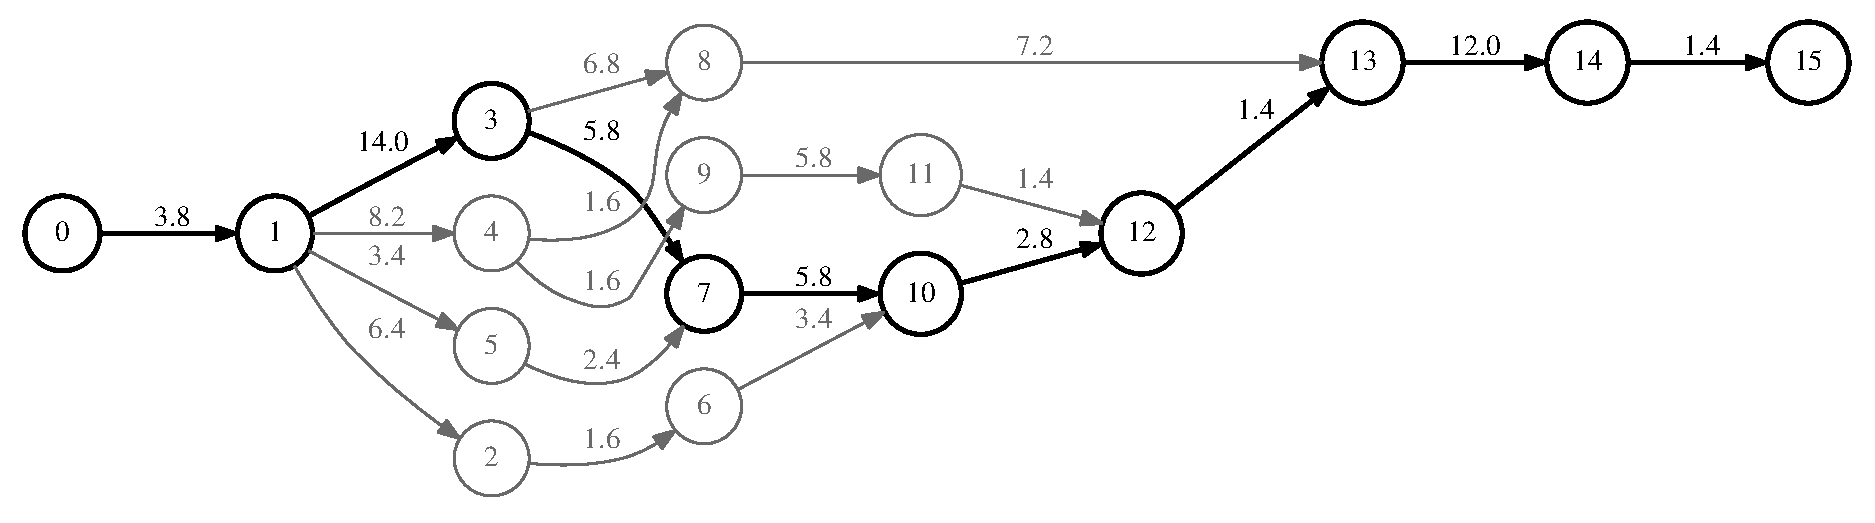
\includegraphics[width=15cm]{./vec/net-model.eps}
\end{dfigure}

Построенный граф состоит из $15$ событий (вершины графа).
Дуги графа --- работы. Каждая дуга графа подписана~сверху соответствующей~ей
продолжительностью работ.

Построенный граф удовлетворяет условию независимости событий $i$ от
события $j$ для все $i > j$. Выполнение этого условия очевидно, так~как~ни одна
дуга не заканчивается в вершине с~номером, меньшим, чем номер вершины
из которой это дуга начиналась. Это позволяет корректно выполнять
дальнейшие расчеты.

\subsubsection{Расчет параметров сетевой модели}

Рассчитаем некоторые характеристики сетевой модели. Характеристики
сетевой модели позволяют определить степень напряженности всего
комплекса работ в целом и~каждой работы в отдельности, а также принять
решение о~перераспределении ресурсов.

Для всех работ рассчитаем следующие показатели:

\begin{itemize}
	\item  ранний срок~начала работы:
		$
			t_{\text{рн}, i - j}  = \max\limits_ {k< i} \left(  t_{\text{ожидаемое}, k - i}  + t_{\text{рн}, k - i} \right)
		$;
	\item ранний срок~окончания работы:
		$
			t_{\text{рo}, i - j}	 = t_{\text{рн}, i - j} + t_{\text{ожидаемое}, i - j} 
		$;
	\item  поздний срок~начала работы: 
		$
			t_{\text{пн}, i - j}	 = t_{\text{по}, i - j} - t_{\text{ожидаемое}, i - j} 
		$;
	\item  поздний срок~окончания работы:
		$
			t_{\text{по}, i - j}  = \min\limits_ {k> j}  \left( t_{\text{по}, j - k} - t_{\text{ожидаемое}, j - k}  \right)
		$;
	\item  полный резерв времени:
		$
			r_{\text{п}, i - j} =t_{\text{пн}, i - j}	 - t_{\text{рн}, i - j}
		$;
	\item  свободный резерв времени: 
		$
			r_{\text{с}, i - j} = t_{\text{рн}, j} - t_{\text{рн}, i} - t_{\text{ожидаемое}, i - j} 
		$.
\end{itemize}

\begin{dsmalltable}{Характеристики сетевой модели, $t$ и~$r$ измеряются в днях.}
	\begin{tabular}{|r|r||r|r||r|r||r|r||r|r|}
		\hline
			Код работы &  $ t_{\text{ож}} $  &
				 $ t_{\text{рн}} $  & $ t_{\text{рo}} $  &
					 $ t_{\text{пн}} $  & $ t_{\text{пo}} $  &
						$ r_{\text{п}} $ & $ r_{\text{с}} $ & 
							$ t_{\text{ож. кр. пути}} $ & $ \delta^2_{\text{кр. пути}}$ \\ 
		\hline
			\textbf{1} &   \textbf{2} & 
				\textbf{3} & \textbf{4} $= 2 + 3$ & 
					\textbf{5} $= 6 - 2$ & \textbf{6} & 
						\textbf{7} $= 5 - 3$ & \textbf{8} & 
							\textbf{9} &  \textbf{10} \\
		\hline 
			\hline  0 --- 1 &$ 3.8$&$ 0.0$&$ 3.8$&$ 0.0$&$ 3.8$&$ 0.0$&$ 0.0 $&$ 3.8$&$0.16$\\
			\hline  1 --- 2 &$ 6.4$&$ 3.8$&$10.2$&$18.0$&$24.4$&$14.2$&$ 0.0 $&$ 0.0$&$0.0 $\\
			\hline  1 --- 3 &$14.0$&$ 3.8$&$17.8$&$ 3.8$&$17.8$&$ 0.0$&$ 0.0 $&$14.0$&$4.0 $\\
			\hline  1 --- 4 &$ 8.2$&$ 3.8$&$12.0$&$15.2$&$23.4$&$11.4$&$ 0.0 $&$ 0.0$&$0.0 $\\
			\hline  1 --- 5 &$ 3.4$&$ 3.8$&$ 7.2$&$17.8$&$21.2$&$14.0$&$ 0.0 $&$ 0.0$&$0.0 $\\
			\hline  2 --- 6 &$ 1.6$&$10.2$&$19.4$&$24.4$&$26.0$&$14.2$&$ 7.6 $&$ 0.0$&$0.0 $\\
			\hline  3 --- 7 &$ 5.8$&$17.8$&$23.6$&$17.8$&$23.6$&$ 0.0$&$ 0.0 $&$ 5.8$&$0.16$\\
			\hline  3 --- 8 &$ 6.8$&$17.8$&$24.6$&$19.6$&$26.4$&$ 1.8$&$ 0.0 $&$ 0.0$&$0.0 $\\
			\hline  4 --- 8 &$ 1.6$&$12.0$&$13.6$&$24.8$&$26.4$&$12.8$&$11.0 $&$ 0.0$&$0.0 $\\
			\hline  4 --- 9 &$ 1.6$&$12.0$&$13.6$&$23.4$&$25.0$&$11.4$&$ 0.0 $&$ 0.0$&$0.0 $\\
			\hline  5 --- 7 &$ 2.4$&$ 7.2$&$ 9.6$&$21.2$&$23.6$&$14.0$&$14.0 $&$ 0.0$&$0.0 $\\
			\hline  6 --- 10&$ 3.4$&$19.4$&$22.8$&$26.0$&$29.4$&$ 6.6$&$ 6.6 $&$ 0.0$&$0.0 $\\
			\hline  7 --- 10&$ 5.8$&$23.6$&$29.4$&$23.6$&$29.4$&$ 0.0$&$ 0.0 $&$ 5.8$&$0.16$\\
			\hline  8 --- 13&$ 7.2$&$24.6$&$31.8$&$26.4$&$33.6$&$ 1.8$&$ 0.4 $&$ 0.0$&$0.0 $\\
			\hline  9 --- 11&$ 5.8$&$13.6$&$19.4$&$25.0$&$30.8$&$11.4$&$ 0.0 $&$ 0.0$&$0.0 $\\
			\hline 10 --- 12&$ 2.8$&$29.4$&$32.2$&$29.4$&$32.2$&$ 0.0$&$ 0.0 $&$ 2.8$&$0.16$\\
			\hline 11 --- 12&$ 1.4$&$19.4$&$20.8$&$30.8$&$32.2$&$11.4$&$11.4 $&$ 0.0$&$0.0 $\\
			\hline 12 --- 13&$ 1.4$&$32.2$&$33.6$&$32.2$&$33.6$&$ 0.0$&$ 0.0 $&$ 1.4$&$0.06$\\
			\hline 13 --- 14&$12.0$&$33.6$&$45.6$&$33.6$&$45.6$&$ 0.0$&$ 0.0 $&$12.0$&$1.0 $\\
			\hline 14 --- 15&$ 1.4$&$45.6$&$47.0$&$45.6$&$47.0$&$ 0.0$&$ 0.0 $&$ 1.4$&$0.06$\\
		\hline	\multicolumn{8}{|r||}{Суммарные время и~дисперсия критического пути:}   &   47.0 &  4.76 \\
		\hline
	\end{tabular} 
\end{dsmalltable}

	
\subsubsection{Анализ сетевой модели}

на~основе посчитанных выше параметров, проведем анализ сетевого
графика. Критически путь включает в себя лишь события с~нулевым запасом времени.
Таким путём является путь из вершин: 
\[
	L_\text{кр} = 0 \rightarrow 1 \rightarrow 3  \rightarrow 7 \rightarrow 10 \rightarrow 12 \rightarrow 13  \rightarrow 14 \rightarrow 15
\]
Суммарное время критического пути составляет $T_\text{кр} = 47$  дней, а его
суммарная дисперсия — $4.76$ дня. 
на~графе критический путь выделен жирными стрелками.

Необходимо, чтобы продолжительность критического пути $T_\text{кр}$
не превышала продолжительности заданного директивного срока $ T_\text{дир}$. 
Если $T_\text{кр} > T_\text{дир}$, то необходимо принять меры по уплотнению графика работ.
В нашем случае директивный срок~создания программного комплекса $T_\text{дир} =63$ дня,\\ 
а продолжительность критического пути $T_\text{кр} = 47$  дней, т.е. $T_\text{кр} < T_\text{дир}$.

Рассчитаем среднеквадратичное отклонение для продолжительности \\
критического пути. 
\[
	\sum\limits_{i-j} \delta^2_{\text{кр. пути}} = 4.76 \Rightarrow  
\]\[
	\Rightarrow  \delta_{\text{кр. пути}} = \sqrt{\sum\limits_{i-j} \delta^2_{\text{кр. пути}}} = \sqrt{4.76} \approx 2.181742422927143
\]

Построим доверительный интервал: 
\[
	\Delta T = T_\text{кр} \pm 3 \cdot \delta_{\text{кр. пути}} = \left[ 40.46; 53.54 \right].
\]

Вычислим вероятность выполнения проекта в директивный срок. Для этого
необходимо определить значение функции Лапласа (по таблице) в точке,
соответствующей директивному сроку:
\[
	P = \varPhi \left( \dfrac{T_\text{дир} - T_\text{кр}}{ \delta_{\text{кр. пути}}} \right) = \varPhi \left( \dfrac{63 - 47}{ 2.18 } \right) = \varPhi(7.334) = 0.999
\]
Таким образом, вероятность завершения работы в  директивный срок~практически равна~$1$, 
то есть проект завершится точно в срок.



\pagebreak
